% !TeX root = ../main.tex
% !TeX encoding = UTF-8
\chapter{Xây dựng quy trình xử lý và trực quan hóa bằng Python}
\label{chap:thuchien}

\section{Quy trình thực hiện tổng thể}

Một biểu đồ đáng tin cậy phải bắt đầu từ một bảng dữ liệu có thể kiểm tra. Với những vấn đề đã khảo sát ở Chương 2, quy trình được tổ chức để mỗi lần biến đổi đều xác định được đầu vào, điều kiện áp dụng và đầu ra. Tệp thô được giữ nguyên; bảng làm việc, dữ liệu sạch và dữ liệu phân tích được lưu riêng. Nhờ vậy, một giá trị trên biểu đồ có thể được đối chiếu ngược với bản ghi nguồn và nhật ký xử lý.

Sáu bước của bài tập được nối thành một luồng thực hiện trong Bảng~\ref{tab:quytrinhpython}. Các thao tác được trình bày tuần tự trong notebook Python, kèm giải thích và kết quả trung gian. Các hàm xử lý phục vụ dashboard được tập hợp thành một mô-đun, tức một bộ mã có chức năng đọc nguồn, làm sạch và tạo biến để ứng dụng có thể thực hiện lại quy trình. Chương này trình bày cách thực hiện cùng một số biểu đồ đại diện; phần phân tích đầy đủ theo Q1--Q5 được trình bày ở Chương 4.

\begin{table}[htbp]
  \centering
  \caption{Tổ chức sáu bước trong quy trình Python}
  \label{tab:quytrinhpython}
  \begingroup
  \small
  \setstretch{1.1}
  \begin{tabularx}{\linewidth}{@{}p{0.95cm}p{3.85cm}Y@{}}
    \toprule
    Bước & Công việc & Đầu ra và điểm kiểm tra \\
    \midrule
    1 & Xác định yêu cầu & Q0--Q5; mẫu số, tiêu chí và sản phẩm cần có. \\
    2 & Đọc, tổ chức nguồn & Bảng thô, hồ sơ nguồn và cấu trúc cột. \\
    3 & Làm sạch, kết hợp & Bảng sạch, nhật ký, khóa ghép và kiểm tra toàn vẹn. \\
    4 & Tạo biến, tính chỉ số & Bảng phân tích và thống kê theo nhóm. \\
    5 & Xây dựng biểu đồ & Hình và bảng hỗ trợ, dùng cùng dữ liệu phân tích. \\
    6 & Xây dựng dashboard & Lọc, hiển thị, tải CSV và cập nhật nguồn. \\
    \bottomrule
  \end{tabularx}
  \endgroup
\end{table}

Các đoạn mã dưới đây chỉ giữ những dòng quyết định phép biến đổi; phần nhập thư viện, khai báo đường dẫn và xuất toàn bộ nhật ký nằm trong mã đầy đủ. Các hình bảng là ảnh chụp cell Python cùng đầu ra Pandas trên giao diện notebook nền tối. Một notebook minh chứng tập hợp các bảng ở từng giai đoạn của quy trình và lượt kiểm tra nội tại bổ sung; các cell chọn một số dòng, cột thực tế để đầu ra đủ rõ khi đưa vào báo cáo. XLSX chỉ đóng vai trò định dạng đầu vào.

\section{Đọc và tổ chức dữ liệu đầu vào}
\label{sec:ch3docdulieu}

Python đọc trang tính dữ liệu chính của nguồn thực hành và bảng tham chiếu UCI. Lựa chọn \maCot{dtype=object} và \maCot{keep_default_na=False} giữ biểu diễn ban đầu, kể cả chuỗi rỗng, trước khi kiểm tra và chuyển kiểu. Trong đoạn mã, \maCot{file_thuc_hanh} và \maCot{file_uci} là hai biến đại diện cho nguồn thực hành và nguồn tham chiếu đã mô tả ở mục~\ref{sec:nguondulieu}; \maCot{ten_trang_du_lieu} chỉ trang tính chứa các bản ghi cần đọc. Những biến này được thiết lập theo nguồn đầu vào khi thực thi. Pandas được nhập với tên \maCot{pd}, NumPy với tên \maCot{np}.

\noindent\begin{minipage}{\linewidth}
\setstretch{1}
\begin{lstlisting}[language=Python]
du_lieu_goc = pd.read_excel(
    file_thuc_hanh, sheet_name=ten_trang_du_lieu,
    dtype=object, keep_default_na=False)
uci_goc = pd.read_csv(file_uci)
du_lieu = du_lieu_goc.copy(deep=True)
du_lieu.insert(0, "Source_Row", np.arange(2, len(du_lieu) + 2))
\end{lstlisting}
\end{minipage}\par

\maCot{Source_Row} lưu số dòng của bảng nguồn, bắt đầu từ 2 vì dòng đầu là tiêu đề. Trường này giữ nguyên qua loại trùng và ghép bảng, giúp tránh nhầm chỉ số DataFrame sau khi sắp xếp với vị trí bản ghi ban đầu. \maCot{Source_File} ghi nhận nguồn xuất xứ; phía UCI có \maCot{Source_Row_UCI} để xác định dòng tham chiếu. Các trường này phục vụ truy vết, không tham gia tính đặc trưng lỗi. Hình~\ref{fig:ch3tho} cho thấy một trích đoạn đầu vào trước khi xử lý. Ô diện tích ở dòng nguồn 7 còn trống; kiểu của các giá trị được đối chiếu ở bước chuẩn hóa tiếp theo.

\begin{center}\begin{minipage}{\linewidth}
  \centering
  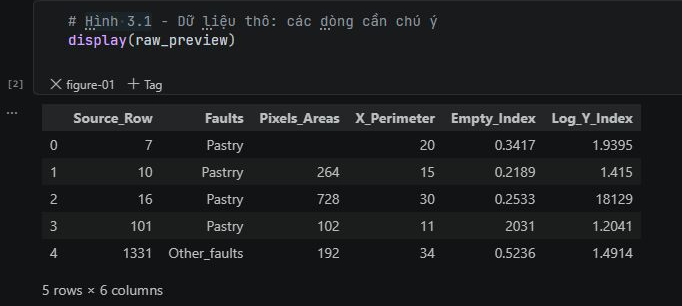
\includegraphics[width=\linewidth]{figures/chuong3/01_du_lieu_tho.png}
  \captionof{figure}{Ảnh cell hiển thị dữ liệu thô trên các dòng nguồn được chọn}
  \label{fig:ch3tho}
\end{minipage}\end{center}

Dữ liệu được tổ chức trong các thư mục tương đối tính từ thư mục gốc của dự án. Thư mục \maCot{data/raw} lưu các nguồn đầu vào; \maCot{data/clean} lưu bảng sau làm sạch; \maCot{data/analysis} lưu bảng đã bổ sung biến phái sinh. Nhật ký xử lý và các bảng kiểm tra được lưu tại \maCot{outputs/buoc_3}; các bảng tổng hợp, hình trực quan và kết quả kiểm thử được tổ chức trong thư mục đầu ra của từng bước tiếp theo. Cách bố trí này giúp đối chiếu các trạng thái dữ liệu và tránh ghi đè nguồn đầu vào.

\section{Thực hiện làm sạch, kết hợp và kiểm chứng dữ liệu}

\subsection{Chuẩn hóa nhãn, kiểu số và loại trùng}

Nhãn được đưa về chữ thường, loại ký tự ngăn cách rồi ánh xạ bằng bảng đã kiểm tra. Chẳng hạn, \maCot{Pastry}, \maCot{Pa stry} và \maCot{Pastrry} cùng được đưa về \maCot{Pastry}; phép ánh xạ xử lý biến thể đã xác nhận, không tự đoán mọi chuỗi gần giống. Quy ước \maCot{K_Scatch} được dùng nhất quán ở bảng phân tích; tên \maCot{K_Scratch} ở nguồn UCI được chuyển theo quy ước này. Mọi nhãn chưa có trong ánh xạ phải được phát hiện trước khi tiếp tục.

Trong đoạn mã sau, \maCot{anh_xa_nhan} là bảng ánh xạ và \maCot{cot_so} là danh sách 27 đặc trưng lấy từ cấu trúc UCI. Khi chuyển kiểu, chuỗi rỗng được xem là thiếu. \maCot{errors="coerce"} chỉ an toàn khi đi cùng kiểm tra thất bại: một chuỗi không rỗng mà không chuyển được không được âm thầm bỏ qua.

\noindent\begin{minipage}{\linewidth}
\setstretch{1}
\begin{lstlisting}[language=Python]
k = du_lieu["Faults"].astype(str).str.lower()
k = k.str.replace(r"[^a-z0-9]", "", regex=True)
du_lieu["Fault_Type_Clean"] = k.map(anh_xa_nhan)
assert du_lieu["Fault_Type_Clean"].notna().all()
for cot in cot_so:
    cu = du_lieu[cot].copy()
    so = pd.to_numeric(cu.mask(cu.eq("")), errors="coerce")
    that_bai = cu.notna() & cu.ne("") & so.isna()
    assert not that_bai.any()
    du_lieu[cot] = so
\end{lstlisting}
\end{minipage}\par

Hình~\ref{fig:ch3chuanhoa} đối chiếu cùng các dòng trước và sau chuẩn hóa. Số biểu diễn nhãn giảm từ 28 về bảy nhãn chuẩn; không có chuỗi số không rỗng nào chuyển đổi thất bại. Những ô vốn trống được giữ là thiếu để xác định căn cứ khôi phục ở bước sau. Trong bảng đối chiếu, \maCot{str} chỉ kiểu chuỗi, \maCot{numeric} chỉ giá trị đã chuyển sang kiểu số; \maCot{NaN} và \maCot{missing} biểu thị giá trị thiếu sau chuyển kiểu.

\begin{center}\begin{minipage}{\linewidth}
  \centering
  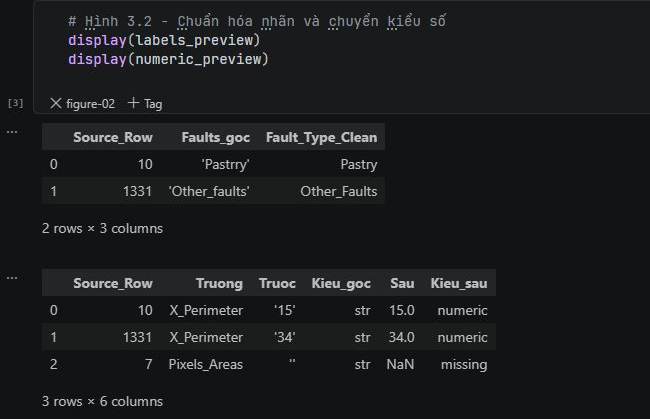
\includegraphics[width=\linewidth]{figures/chuong3/02_chuan_hoa.png}
  \captionof{figure}{Ảnh cell đối chiếu nhãn và kiểu số trước, sau chuẩn hóa}
  \label{fig:ch3chuanhoa}
\end{minipage}\end{center}

Trùng lặp được xác định sau chuẩn hóa theo 27 đặc trưng, ngày gốc và nhãn chuẩn. Chỉ có chung tọa độ chưa đủ để loại một dòng nếu các trường còn lại khác nhau. Mã giữ lần xuất hiện đầu tiên; nhật ký lưu cả \maCot{Source_Row} của dòng loại và \maCot{Kept_Source_Row} của dòng giữ. Cờ \maCot{bi_trung} được tính trước khi lọc để thông tin này không bị mất.

\noindent\begin{minipage}{\linewidth}
\setstretch{1}
\begin{lstlisting}[language=Python]
tieu_chi = cot_so + ["Production_Date", "Fault_Type_Clean"]
bi_trung = du_lieu.duplicated(tieu_chi, keep="first")
du_lieu = du_lieu.loc[~bi_trung].copy()
\end{lstlisting}
\end{minipage}\par

Hình~\ref{fig:ch3trung} minh họa các cặp dòng giữ--loại được ghi trong nhật ký loại trùng. Sau thao tác này, 1.961 dòng còn 1.941 dòng; tổng ô thiếu trong 27 đặc trưng giảm từ 70 xuống 67. Ba ô thiếu không cần điền nữa thuộc các bản sao đã loại, vì vậy số khôi phục không được lấy trực tiếp từ tổng thiếu ban đầu.

\begin{center}\begin{minipage}{\linewidth}
  \centering
  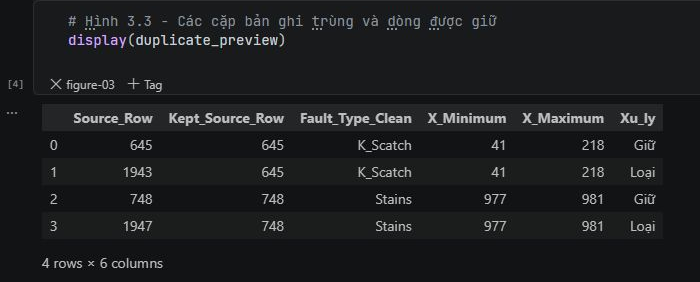
\includegraphics[width=\linewidth]{figures/chuong3/03_loai_trung.png}
  \captionof{figure}{Ảnh cell hiển thị các cặp bản ghi trùng và dòng được giữ}
  \label{fig:ch3trung}
\end{minipage}\end{center}

\subsection{Kiểm tra nội tại trước khôi phục}
\label{sec:ch3kiemtranoitai}

Phép kiểm tra nội tại sử dụng bảng đã chuẩn hóa và loại trùng, trước khi lấy giá trị UCI để điền hoặc sửa. Trong notebook, kiểm tra công thức được thực hiện sau khôi phục. Vì vậy, bài bổ sung một lượt rà soát trên bảng chưa khôi phục để xác định những sai lệch có thể phát hiện từ quan hệ giữa các cột. Các hình và số đếm ở giai đoạn này sử dụng kết quả rà soát bổ sung, được ghi riêng với kết quả đối chiếu nguồn.

Các quan hệ làm việc gồm \maCot{Empty_Index} với diện tích và khung bao, \maCot{Log_Y_Index} với khoảng tọa độ Y, \maCot{LogOfAreas} với diện tích và \maCot{Orientation_Index} với hai kích thước khung bao. Chúng đã được đối chiếu trong quy trình, nhưng không được coi là định nghĩa chính thức do metadata UCI cung cấp. Mã minh họa dưới đây giữ một quan hệ tiêu biểu; \maCot{du_lieu} vẫn là bảng chưa khôi phục.

\noindent\begin{minipage}{\linewidth}
\setstretch{1}
\begin{lstlisting}[language=Python]
dx = du_lieu["X_Maximum"] - du_lieu["X_Minimum"]
dy = du_lieu["Y_Maximum"] - du_lieu["Y_Minimum"]
du_kien = 1 - du_lieu["Pixels_Areas"] / (dx * dy)
du_dieu_kien = du_lieu["Empty_Index"].notna()
du_dieu_kien &= du_kien.notna() & np.isfinite(du_kien)
sai_lech = (du_lieu["Empty_Index"] - du_kien.round(4)).abs()
gan_co = du_dieu_kien & sai_lech.gt(0.00010001)
\end{lstlisting}
\end{minipage}\par

Điều kiện đủ toán hạng và hữu hạn loại khỏi phép kiểm tra những trường hợp chưa tính được giá trị dự kiến. Dung sai xét đến độ chính xác làm tròn của chỉ số. Hình~\ref{fig:ch3noitai} thể hiện giá trị trong tệp và giá trị tính từ những cột cùng dòng; chưa sử dụng giá trị tham chiếu để tạo dấu hiệu phát hiện.

\begin{center}\begin{minipage}{\linewidth}
  \centering
  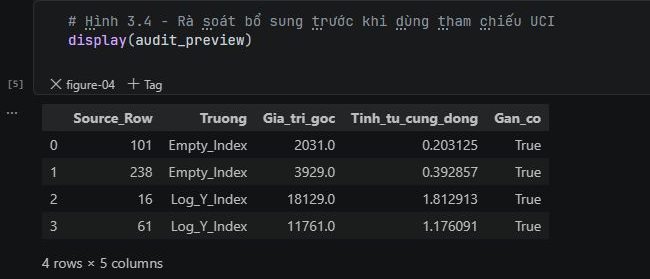
\includegraphics[width=\linewidth]{figures/chuong3/04_kiem_tra_noi_tai.png}
  \captionof{figure}{Ảnh cell kiểm tra nội tại bổ sung trên bảng chưa khôi phục}
  \label{fig:ch3noitai}
\end{minipage}\end{center}

Lượt kiểm tra bổ sung gắn cờ 16 ô: mười ô \maCot{Empty_Index} và sáu ô \maCot{Log_Y_Index}. Một ô có thể vi phạm cả miền giá trị lẫn quan hệ phái sinh; tổng được tính theo cặp dòng--trường duy nhất. Mã chạy lại \maCot{kiem_tra_q0_truoc_tham_chieu.py}, bảng ô vi phạm và bản tóm tắt được lưu tại \maCot{outputs/ra_soat_de_cuong}. Đối chiếu sau khi phát hiện cho thấy 16 cặp dòng--trường này trùng đúng 16 ô trong nhật ký sửa theo UCI. Cờ chỉ xác định vị trí cần xem xét. Giá trị thay thế vẫn phải có căn cứ riêng, được xác nhận khi ghép với nguồn tương ứng.

\subsection{Ghép UCI và khôi phục có truy vết}

Bốn trường \maCot{X_Minimum}, \maCot{X_Maximum}, \maCot{Y_Minimum}, \maCot{Y_Maximum} được chọn làm \maCot{khoa_ghep} sau khi kiểm tra ở cả hai bảng: không thiếu, có giá trị nguyên và không trùng tổ hợp khóa. Bảng \maCot{tham_chieu} chứa 27 đặc trưng, dòng UCI và nhãn suy ra từ bảy cột one-hot; mỗi dòng nguồn phải có đúng một cờ nhãn bằng 1. Các điều kiện này bảo vệ phép ghép khỏi nhân bản bản ghi hoặc chọn nhầm nguồn.

\noindent\begin{minipage}{\linewidth}
\setstretch{1}
\begin{lstlisting}[language=Python]
du_lieu_ghep = du_lieu.merge(
    tham_chieu, on=khoa_ghep, how="left",
    suffixes=("", "_UCI"), validate="one_to_one", indicator=True)
assert du_lieu_ghep["_merge"].eq("both").all()
assert du_lieu_ghep["Fault_Type_Clean"].eq(
    du_lieu_ghep["Fault_Type_UCI"]).all()
\end{lstlisting}
\end{minipage}\par

\maCot{validate="one_to_one"} yêu cầu quan hệ một--một; \maCot{indicator=True} cho phép kiểm tra dòng khớp và chưa khớp~\cite{pandasmerge}. Chỉ khi toàn bộ bản ghi ghép được và nhãn tương ứng nhất quán, giá trị tham chiếu mới được dùng. Hình~\ref{fig:ch3khoiphuc} minh họa ô thiếu và ô có giá trị khác nguồn, cùng vị trí dòng UCI đã xác định.

\begin{center}\begin{minipage}{\linewidth}
  \centering
  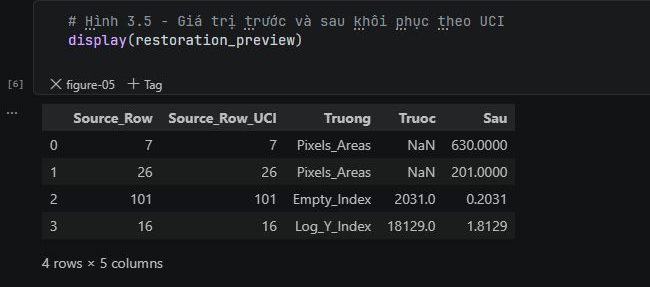
\includegraphics[width=\linewidth]{figures/chuong3/05_khoi_phuc_uci.png}
  \captionof{figure}{Ảnh cell trích nhật ký khôi phục và sửa giá trị theo UCI}
  \label{fig:ch3khoiphuc}
\end{minipage}\end{center}

Hai thao tác được phân biệt trong nhật ký: khôi phục ô đang thiếu và sửa ô có giá trị khác nguồn. Ví dụ, \maCot{Pixels_Areas} tại dòng nguồn 7 được khôi phục thành 630; \maCot{Empty_Index} tại dòng 101 được sửa từ 2031 thành 0,2031. Giá trị sau lấy từ UCI tại khóa đã ghép, không suy đoán bằng cách dịch dấu thập phân. Đoạn mã sau minh họa một trường \maCot{cot} không thuộc khóa; mã đầy đủ bổ sung loại thao tác và căn cứ trước khi ghép nhật ký của các trường.

\noindent\begin{minipage}{\linewidth}
\setstretch{1}
\begin{lstlisting}[language=Python]
cu = du_lieu_ghep[cot].copy()
moi = du_lieu_ghep[cot + "_UCI"]
thieu = cu.isna()
khac = ~thieu & ~np.isclose(cu, moi, rtol=0, atol=1e-9)
doi = thieu | khac
nhat_ky = du_lieu_ghep.loc[doi,
    ["Source_Row", "Source_Row_UCI"]].copy()
nhat_ky["Truong"] = cot
nhat_ky["Gia_tri_truoc"] = cu[doi]
nhat_ky["Gia_tri_sau"] = moi[doi]
du_lieu_ghep.loc[doi, cot] = moi[doi]
\end{lstlisting}
\end{minipage}\par

Quy trình khôi phục 67 ô thiếu và sửa 16 giá trị số. Các ví dụ ở Hình~\ref{fig:ch3khoiphuc} được trích từ nhật ký khôi phục ô thiếu và nhật ký sửa giá trị; mỗi mục ghi dòng nguồn, dòng tham chiếu, trường thay đổi và giá trị trước--sau. Sau xử lý, 52.407 ô đặc trưng được đối chiếu với nguồn tham chiếu. Độ khớp này xác nhận đúng phép ghép và thao tác khôi phục; do UCI đã cung cấp giá trị thay thế, nó không phải thước đo độc lập về khả năng phát hiện sai sót. Nhật ký phát hiện trước tham chiếu và nhật ký thay đổi được giữ riêng để kiểm tra hai hoạt động này.

\subsection{Chuẩn hóa ngày, gắn cờ diện tích và kiểm tra đầu ra}

Ngày gốc được giữ trong \maCot{Production_Date}; ngày chuẩn lưu ở \maCot{Production_Date_Clean}, kèm cờ \maCot{Date_Is_Simulated} để nhận biết ngày mô phỏng. Hàm \maCot{clean_simulated_date} chuẩn hóa các cách biểu diễn ngày theo lịch mô phỏng gồm các ngày 2, 3, 10, 21 và 30 tháng 11 năm 2025. Ví dụ, giá trị đầu vào tại dòng 2 là 2025-02-11 được chuyển thành 2025-11-02 theo lịch đã biết. Đây là quy tắc riêng của dữ liệu thực hành, không phải cách đảo ngày/tháng áp dụng cho mọi dữ liệu. Chuẩn hóa phục vụ tính nhất quán và truy vết; ngày này không được dùng để phân tích xu hướng sản xuất.

\noindent\begin{minipage}{\linewidth}
\setstretch{1}
\begin{lstlisting}[language=Python]
du_lieu_ghep["Production_Date_Clean"] = pd.to_datetime(
    du_lieu_ghep["Production_Date"].map(clean_simulated_date))
du_lieu_ghep["Date_Is_Simulated"] = True
area = du_lieu_ghep["Pixels_Areas"]
q1, q3 = area.quantile([0.25, 0.75])
du_lieu_ghep["Area_Outlier_Flag"] = (
    area.lt(q1 - 1.5 * (q3 - q1)) | area.gt(q3 + 1.5 * (q3 - q1)))
\end{lstlisting}
\end{minipage}\par

Cờ diện tích được tính trên toàn bộ 1.941 dòng đã khôi phục theo hàng rào $1{,}5\times\mathrm{IQR}$. Có 395 dòng được gắn cờ và giữ lại. Cờ toàn tập này phục vụ xem xét dữ liệu; các điểm ngoài râu ở boxplot Q5 được tính lại trong từng nhóm, nên hai số đếm không đồng nghĩa. Theo nguyên tắc ở Chương 1, diện tích lớn chưa đủ căn cứ xác định sai dữ liệu~\cite{nistbox}.

Trước khi xuất bảng sau làm sạch, quy trình kiểm tra số dòng, nhãn hợp lệ, không thiếu đặc trưng, cờ dòng thép, quan hệ tọa độ, miền độ sáng và các công thức làm việc. Bảng được lưu ở định dạng CSV rồi đọc lại để đối chiếu dữ liệu số và nhãn; ngày được phân tích về kiểu ngày khi cần so sánh. Tùy chọn \maCot{index=False} tránh xuất thêm chỉ số dòng của DataFrame; mã hóa \maCot{utf-8-sig} hỗ trợ lưu chữ tiếng Việt. Kiểm tra sau xuất bảo đảm bảng giao cho bước phân tích giữ đúng giá trị đã xử lý.

\section{Tạo biến phái sinh và các bảng thống kê}

Bảng phân tích được tạo từ bản sao bảng sau làm sạch. Trong mã minh họa, \maCot{loi_thep_sach} đại diện cho bảng sau làm sạch và \maCot{d} là tên viết gọn của bảng phân tích. Trước khi tổng hợp cột dòng thép \maCot{Steel_Type}, hai cờ A300/A400 được kiểm tra chỉ nhận 0 hoặc 1 và có tổng bằng 1 trên mỗi dòng. Kích thước, diện tích và độ dày phải dương; độ sáng tối đa không được nhỏ hơn tối thiểu. Những điều kiện này cần đạt trước khi lấy hiệu hoặc logarit.

\noindent\begin{minipage}{\linewidth}
\setstretch{1}
\begin{lstlisting}[language=Python]
d = loi_thep_sach.copy(deep=True)
d["Steel_Type"] = np.where(
    d["TypeOfSteel_A300"].eq(1), "A300", "A400")
d["X_Range"] = d["X_Maximum"] - d["X_Minimum"]
d["Y_Range"] = d["Y_Maximum"] - d["Y_Minimum"]
d["Luminosity_Range"] = (
    d["Maximum_of_Luminosity"] - d["Minimum_of_Luminosity"])
d["Log_Pixels_Areas"] = np.log10(d["Pixels_Areas"].astype(float))
\end{lstlisting}
\end{minipage}\par

Hình~\ref{fig:ch3phantich} minh họa các trường bổ sung trên những bản ghi thực tế, cùng ngày chuẩn và cờ mô phỏng. \maCot{X_Range} và \maCot{Y_Range} mô tả kích thước khung bao, không thay thế diện tích vùng lỗi. \maCot{Luminosity_Range} là hiệu độ sáng tối đa--tối thiểu; chưa có căn cứ đồng nhất nó với \maCot{Luminosity_Index}. \maCot{Log_Pixels_Areas} dùng cơ số 10 và tính lại thông tin đã có trong \maCot{LogOfAreas}; sai khác được kiểm tra trong dung sai 0,00010001 do làm tròn. Cột này hỗ trợ kiểm chứng, không tăng số đặc trưng độc lập.

\begin{center}\begin{minipage}{\linewidth}
  \centering
  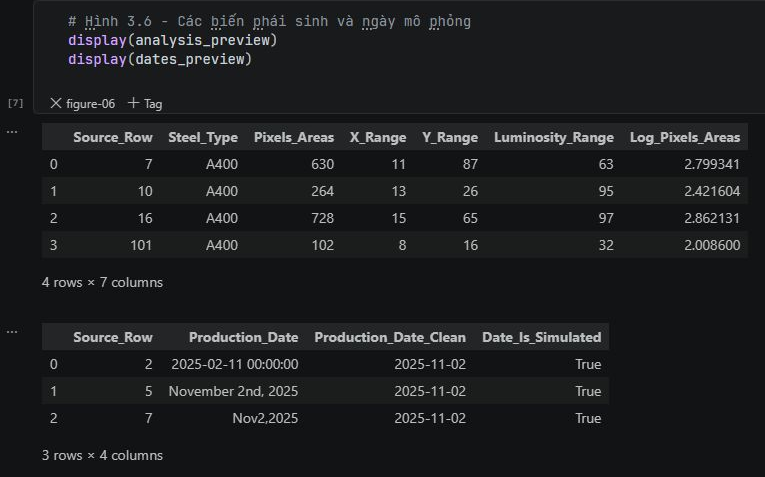
\includegraphics[width=\linewidth]{figures/chuong3/06_du_lieu_phan_tich.png}
  \captionof{figure}{Ảnh cell hiển thị biến phái sinh và ngày mô phỏng sau chuẩn hóa}
  \label{fig:ch3phantich}
\end{minipage}\end{center}

Các bảng thống kê được tính trực tiếp từ bảng phân tích. Q1 dùng số đếm giảm dần, tỷ trọng và lũy kế. Q2 bắt đầu từ bảng chéo nhãn--dòng thép; chuẩn hóa theo cột cho cơ cấu nhãn trong dòng thép, chuẩn hóa theo hàng cho phân bố dòng thép trong từng nhãn. Hai tỷ trọng được lưu thành hai trường riêng trong bảng thống kê; mã minh họa dưới đây thể hiện phép chia theo hai chiều.

\noindent\begin{minipage}{\linewidth}
\setstretch{1}
\begin{lstlisting}[language=Python]
dem = pd.crosstab(d["Fault_Type_Clean"], d["Steel_Type"])
trong_dong_thep = dem.div(dem.sum(axis=0), axis=1) * 100
trong_nhan = dem.div(dem.sum(axis=1), axis=0) * 100
g = d.groupby("Fault_Type_Clean")["Pixels_Areas"]
thong_ke = g.agg(N="count", Median="median", SD="std")
thong_ke["P25"] = g.quantile(0.25)
thong_ke["P75"] = g.quantile(0.75)
thong_ke["IQR"] = thong_ke["P75"] - thong_ke["P25"]
\end{lstlisting}
\end{minipage}\par

Mã minh họa thống kê diện tích được áp dụng tương tự cho độ sáng và độ dày; bổ sung min/max khi xuất bảng. Độ dày còn được nhóm theo nhãn và dòng thép để so sánh trong cùng nhãn. \maCot{std} sử dụng độ lệch chuẩn mẫu với mẫu số $N-1$; nhóm $N=1$ giữ kết quả chưa xác định, không điền 0. Với dashboard, dòng thép không có quan sát sau lọc cũng chưa có tỷ trọng. Bảng thống kê và biểu đồ đều phải giữ cỡ mẫu tương ứng với phạm vi đang xét.

\section{Xây dựng biểu đồ theo câu hỏi phân tích}

Biểu đồ được dựng từ bảng phân tích và các bảng tổng hợp đã kiểm tra, không tính lại trên nguồn thô. Ba hình dưới đây minh họa trực tiếp cách chuyển số liệu thành biểu đồ cơ cấu, quan hệ giữa hai biến và phân bố theo nhóm. Mã được rút gọn để làm rõ thao tác chính; tiêu đề, nhãn trục, cỡ mẫu, màu và chú thích nguồn được bổ sung trong mã đầy đủ. \maCot{MAU_LOI} là bảng màu gắn cố định với bảy nhãn, được dùng thống nhất giữa các hình.

Những hình còn lại được tổ chức theo cùng nguyên tắc. Q2 dùng số đếm cho cột nhóm, còn cột 100\% dùng tỷ trọng trong từng dòng thép; bảng tỷ trọng trong nhãn cung cấp căn cứ đọc ngưỡng trên 90\%. Q4 dùng boxplot độ dày và bảng nhãn--dòng thép. Mỗi hình phải ghi rõ phạm vi và giữ cỡ mẫu khi so sánh.

\subsection{Biểu đồ cơ cấu và tỷ trọng lũy kế}

Thanh ngang và Pareto ở Q1 cùng sử dụng thứ tự số đếm giảm dần. Trong Pareto, cột biểu diễn số bản ghi, còn đường biểu diễn tỷ trọng lũy kế trên tổng bản ghi lỗi. Hai đại lượng dùng hai trục tung riêng. Mốc 80\% được vẽ ở trục phần trăm để đọc mức tập trung trong mẫu.

\noindent\begin{minipage}{\linewidth}
\setstretch{1}
\begin{lstlisting}[language=Python]
dem = d["Fault_Type_Clean"].value_counts()
luy_ke = dem.cumsum() / dem.sum() * 100
fig, ax = plt.subplots(figsize=(11, 6))
ax.bar(dem.index, dem, color=[MAU_LOI[n] for n in dem.index])
ax_luy_ke = ax.twinx()
ax_luy_ke.plot(dem.index, luy_ke, marker="o", color="black")
ax_luy_ke.axhline(80, linestyle="--", color="gray")
ax_luy_ke.set_ylim(0, 105)
\end{lstlisting}
\end{minipage}\par

Hình~\ref{fig:ch3pareto} là sản phẩm từ mã vẽ đầy đủ trên 1.941 bản ghi sau xử lý. Nhãn phần trăm nằm trên đường lũy kế; tên loại lỗi được xoay để tránh chồng chữ. Chú thích phân biệt số lượng với phần trăm, giúp người đọc theo dõi đúng mẫu số khi đối chiếu bảng cơ cấu.

\begin{center}\begin{minipage}{\linewidth}
  \centering
  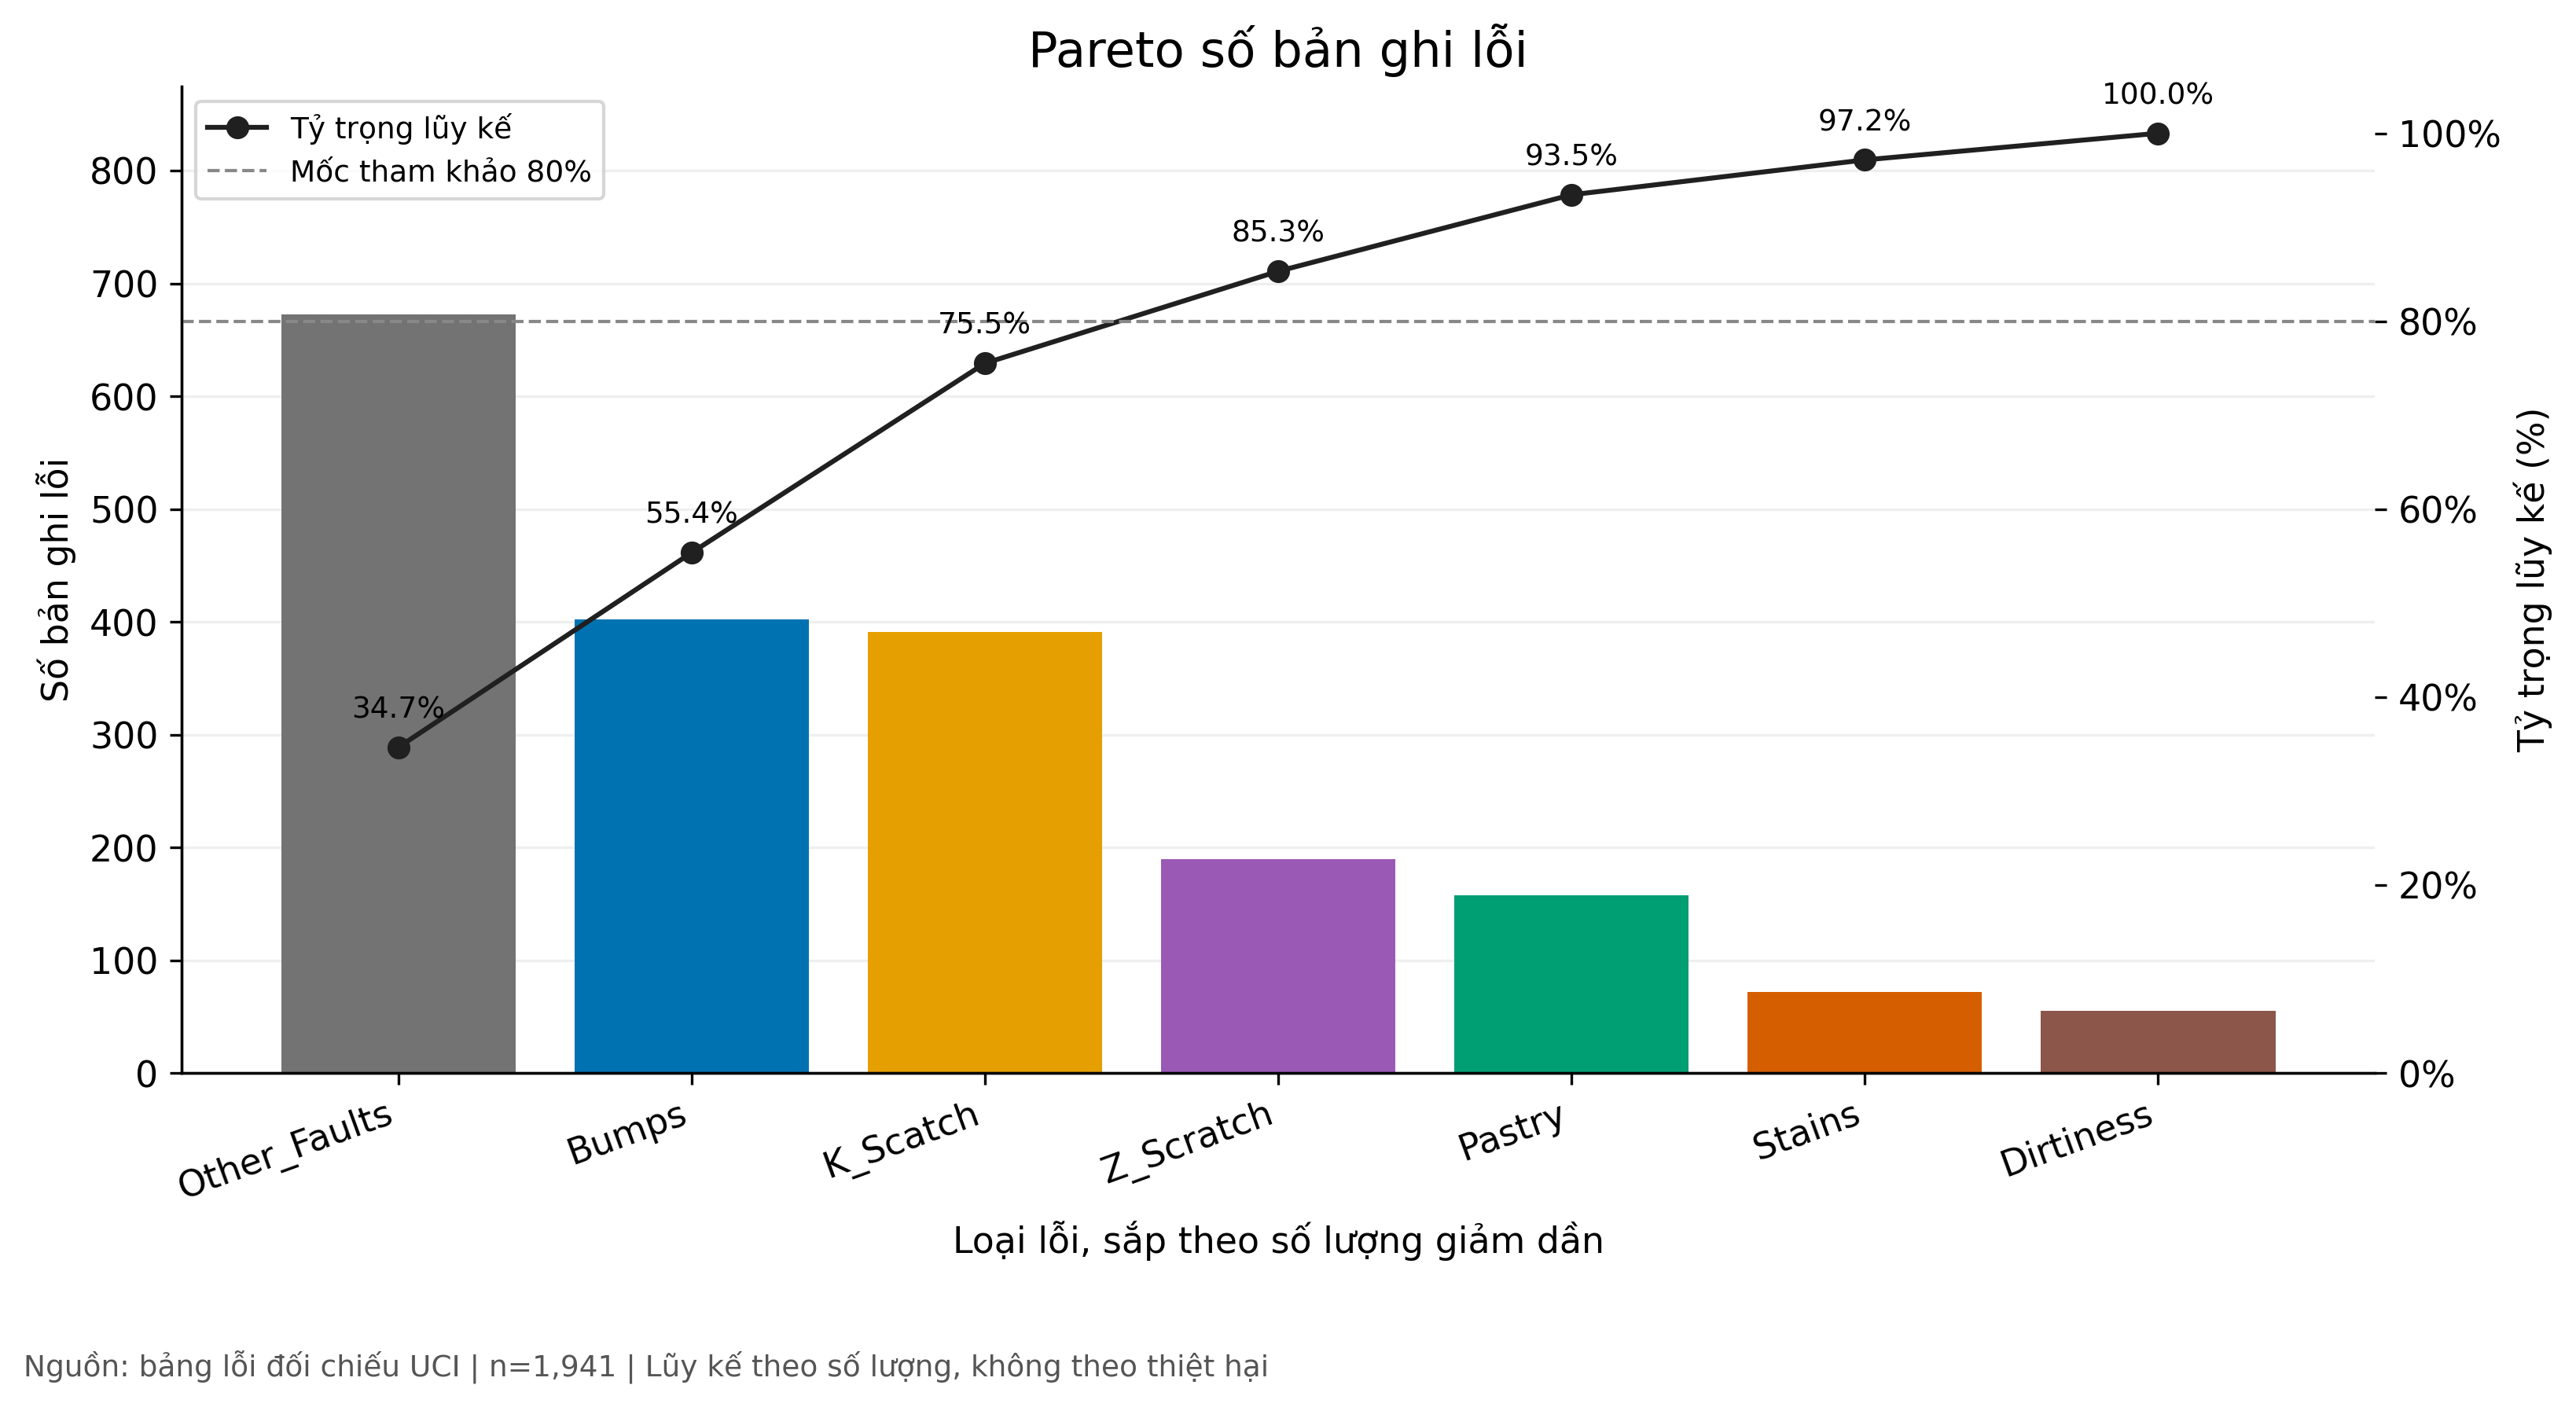
\includegraphics[width=\linewidth]{figures/chuong3/07_pareto_loi.png}
  \captionof{figure}{Minh họa Pareto từ bảng số đếm và tỷ trọng lũy kế của các nhãn lỗi}
  \label{fig:ch3pareto}
\end{minipage}\end{center}

\subsection{Biểu đồ phân tán độ sáng theo nhãn}

Q3 đặt độ sáng tối thiểu trên trục ngang và tối đa trên trục dọc. Mỗi bản ghi tạo một điểm; nhóm nhãn quyết định màu. Tham số \maCot{alpha=0.35} giảm độ đậm để các vùng có nhiều điểm chồng lên nhau vẫn đọc được. Không nối các điểm, vì dữ liệu không biểu diễn một chuỗi có thứ tự.

\noindent\begin{minipage}{\linewidth}
\setstretch{1}
\begin{lstlisting}[language=Python]
fig, ax = plt.subplots(figsize=(11, 7))
for nhan, nhom in d.groupby("Fault_Type_Clean"):
    ax.scatter(
        nhom["Minimum_of_Luminosity"],
        nhom["Maximum_of_Luminosity"],
        s=22, alpha=0.35, color=MAU_LOI[nhan],
        edgecolors="none", label=f"{nhan} (n={len(nhom)})")
ax.legend(title="Loai loi", bbox_to_anchor=(1.02, 1))
\end{lstlisting}
\end{minipage}\par

Hình~\ref{fig:ch3scatter} giữ toàn bộ bản ghi, ghi cỡ mẫu từng nhãn trong chú giải và sử dụng thang độ sáng theo nguồn. Hệ số Pearson trong tiêu đề là thông tin bổ trợ về quan hệ giữa hai biến. Nhận xét vùng trung tâm cần đối chiếu thêm P25/P75 theo tiêu chí tại mục~\ref{sec:yeucauphanTich}, vì độ trong suốt và sự chồng điểm chưa thay thế được bảng thống kê.

\begin{center}\begin{minipage}{\linewidth}
  \centering
  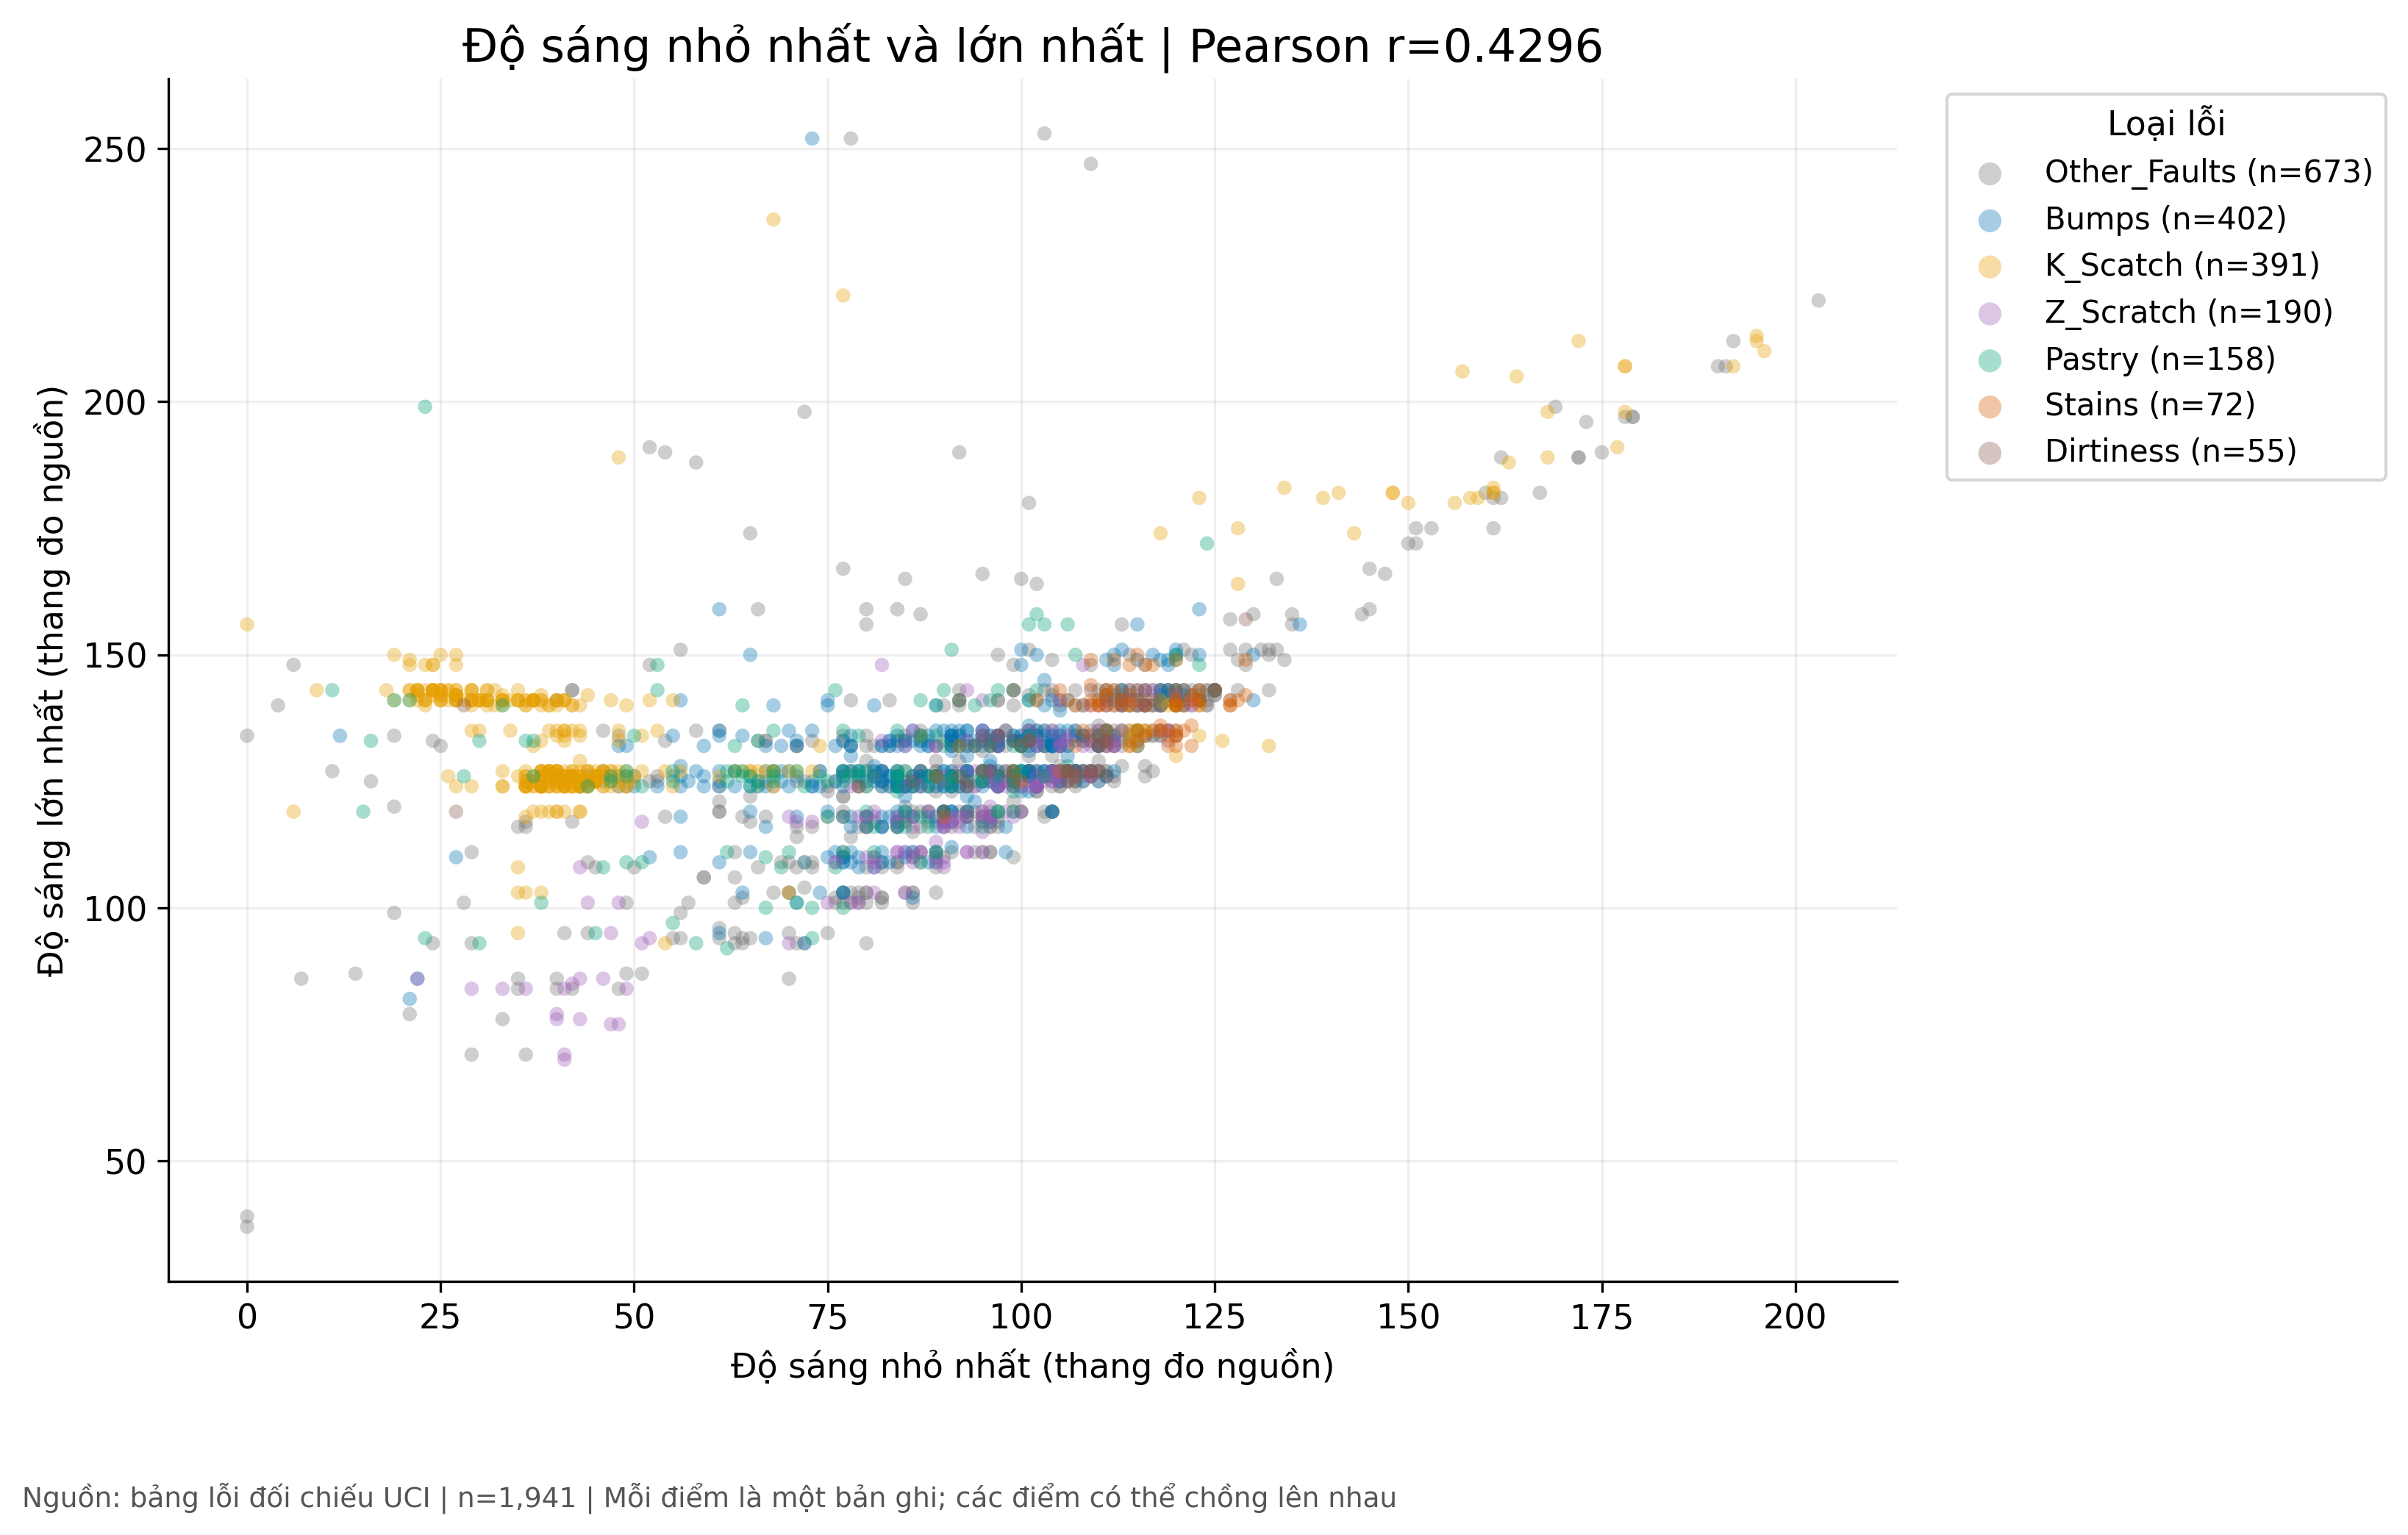
\includegraphics[width=\linewidth]{figures/chuong3/08_scatter_do_sang.png}
  \captionof{figure}{Minh họa scatter độ sáng tối thiểu--tối đa, phân biệt nhãn bằng màu và cỡ mẫu}
  \label{fig:ch3scatter}
\end{minipage}\end{center}

\subsection{Boxplot diện tích trên trục logarit}

Q5 giữ diện tích gốc để tính hộp, râu và điểm ngoài râu, sau đó mới đổi trục hiển thị sang log. Các nhãn được xếp cùng thứ tự với bảng cơ cấu; hộp nằm ngang để đọc rõ tên nhóm và cỡ mẫu. Điều kiện diện tích dương đã được kiểm tra ở bước tạo bảng phân tích.

\noindent\begin{minipage}{\linewidth}
\setstretch{1}
\begin{lstlisting}[language=Python]
nhan = d["Fault_Type_Clean"].value_counts().index.tolist()
mau = [d.loc[d["Fault_Type_Clean"].eq(n), "Pixels_Areas"]
       for n in nhan]
fig, ax = plt.subplots(figsize=(10, 5))
ax.boxplot(mau, vert=False, whis=1.5, showfliers=True)
ax.set_yticks(range(1, len(nhan) + 1), nhan)
ax.invert_yaxis()
ax.set_xscale("log")
\end{lstlisting}
\end{minipage}\par

Hình~\ref{fig:ch3boxarea} là đầu ra hoàn chỉnh tương ứng với đoạn mã minh họa. \maCot{set_xscale("log")} thay cách hiển thị sau khi hộp đã được tính từ \maCot{Pixels_Areas}; nó không thay dữ liệu đầu vào thành cột logarit. Nhãn trục vẫn ghi diện tích gốc. Các điểm ngoài râu được giữ và tính theo từng nhãn, khác với cờ IQR toàn tập ở bước làm sạch.

\begin{center}\begin{minipage}{\linewidth}
  \centering
  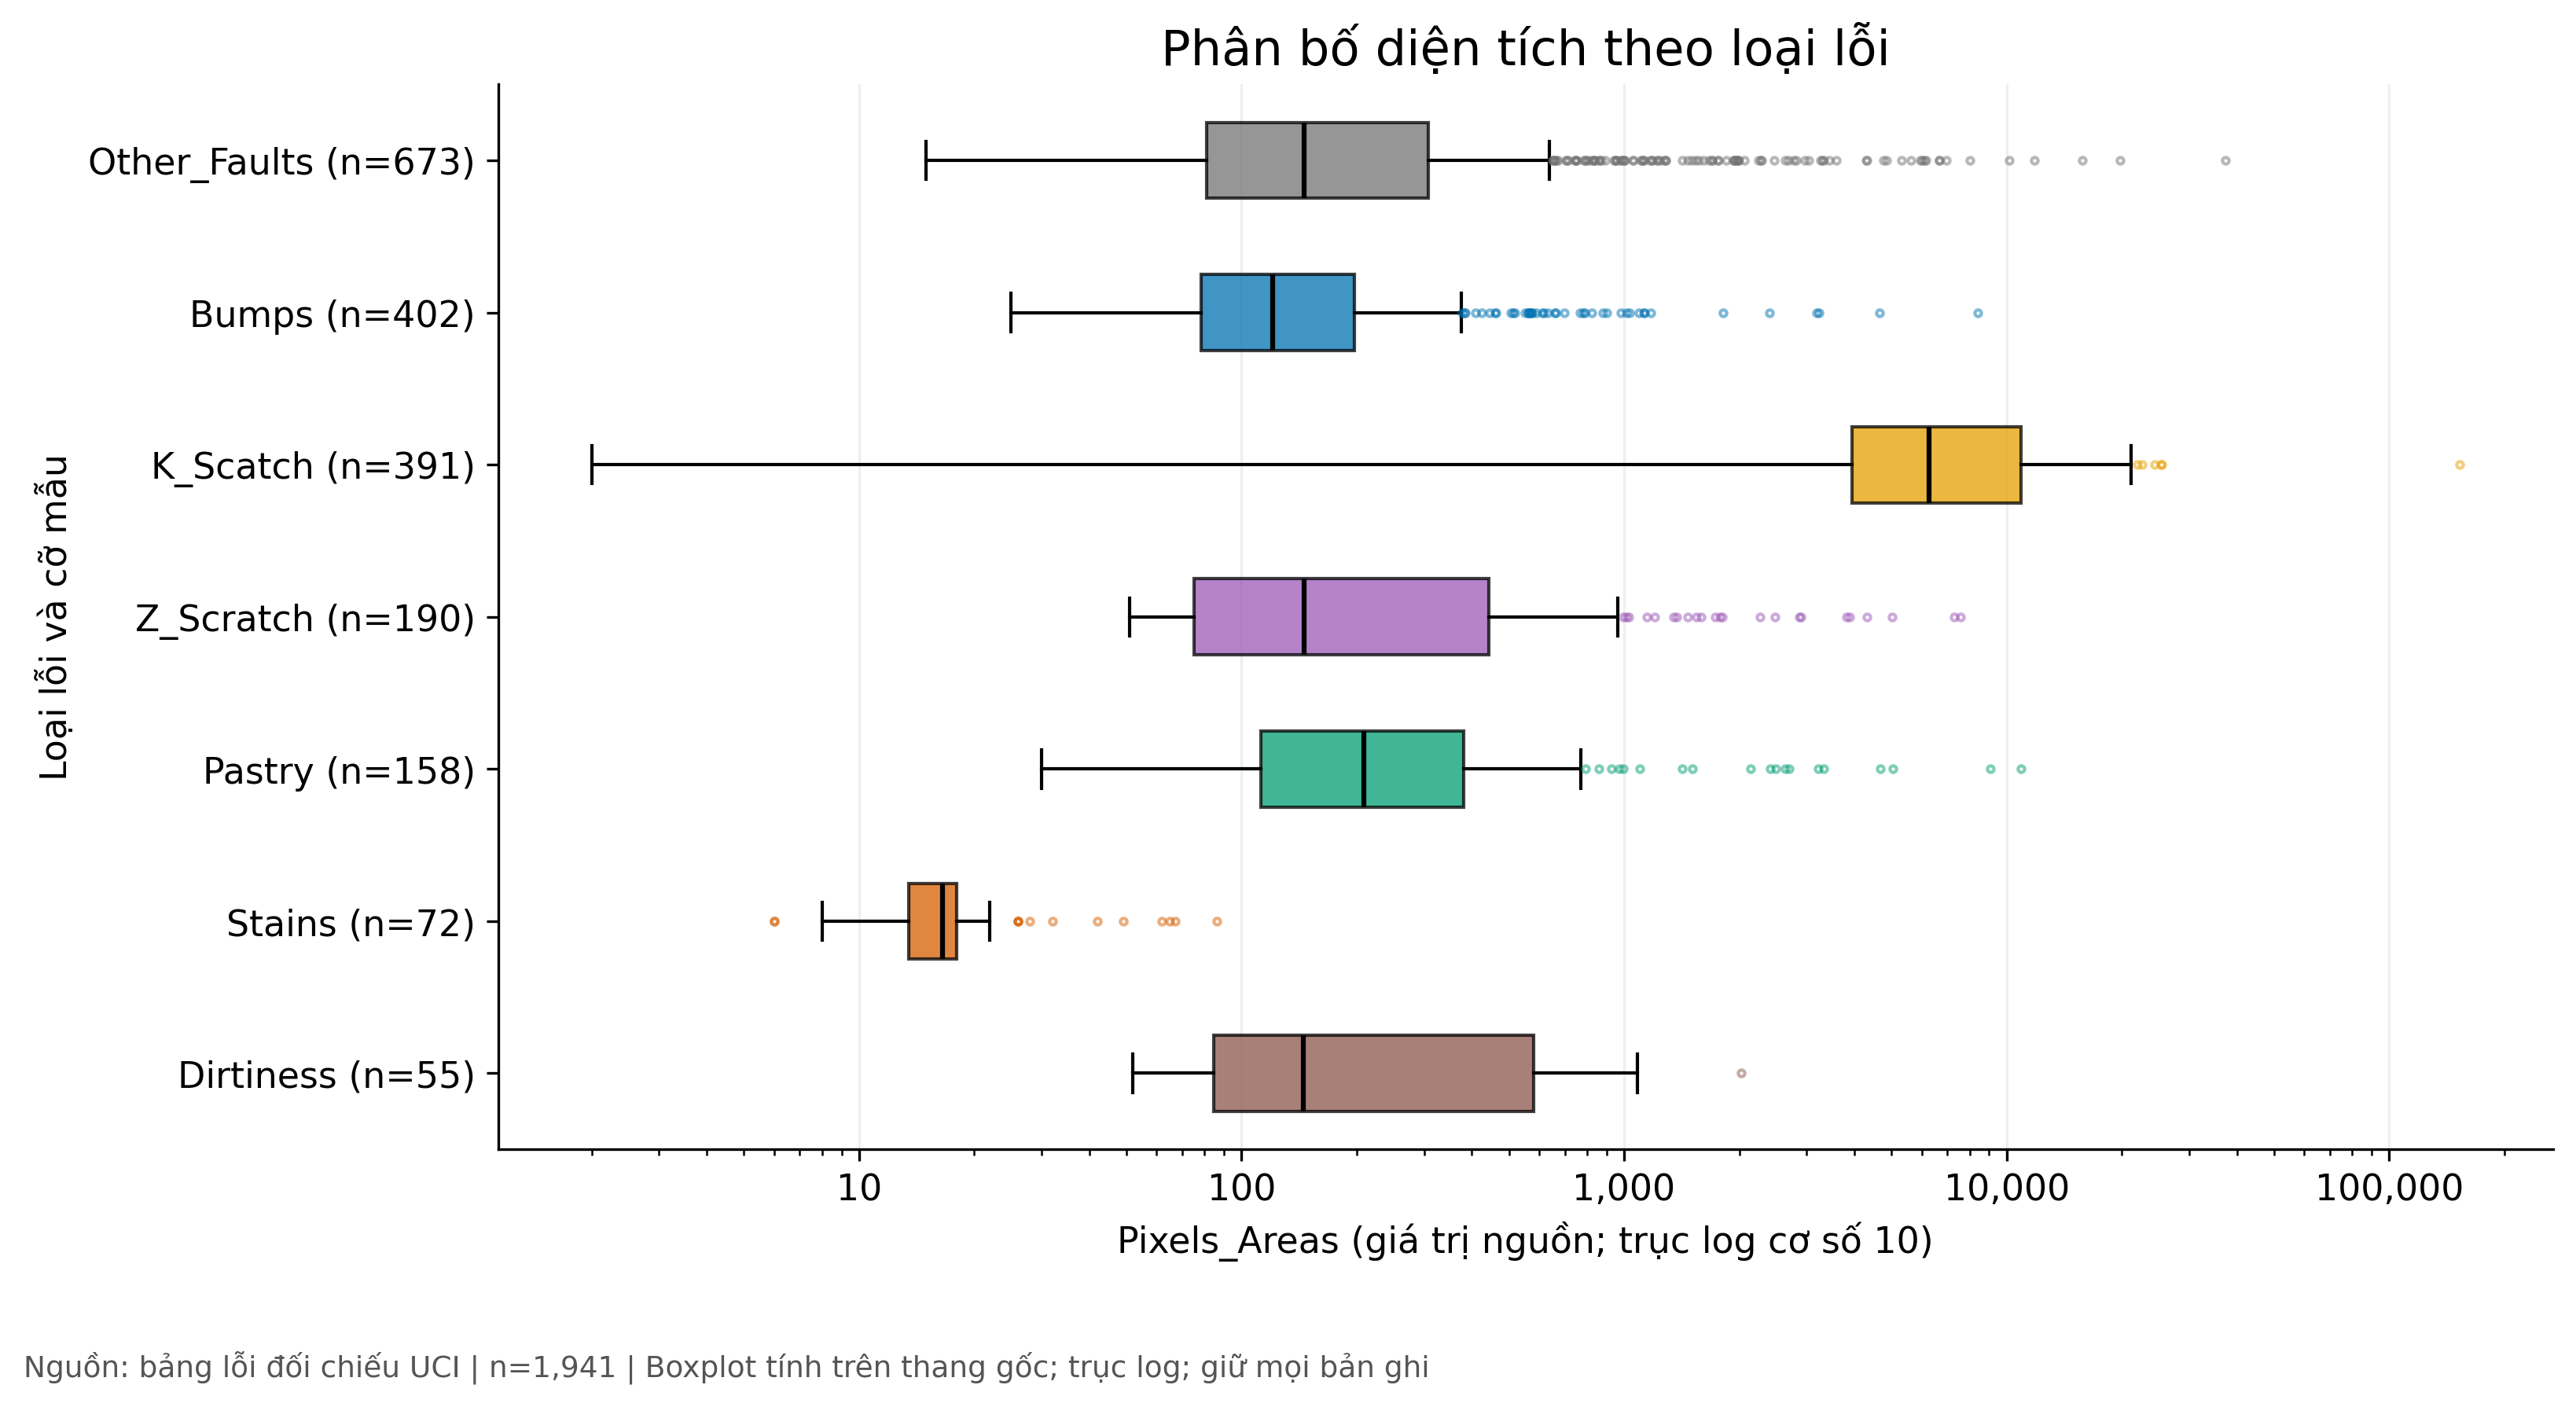
\includegraphics[width=\linewidth]{figures/chuong3/09_boxplot_dien_tich_log.png}
  \captionof{figure}{Minh họa boxplot tính trên diện tích gốc rồi hiển thị với trục log cơ số 10}
  \label{fig:ch3boxarea}
\end{minipage}\end{center}

Các hình được xuất PNG độ phân giải 300 dpi và SVG để có thể đưa vào báo cáo với chữ rõ~\cite{matplotlib}. Bảng hỗ trợ được xuất CSV cùng giai đoạn, giúp đối chiếu hình với số liệu. Các minh họa ở mục này thể hiện cách dựng và quy tắc hiển thị; phần trả lời đầy đủ Q1--Q5 được triển khai ở Chương 4.

\section{Xây dựng dashboard tương tác}

\subsection{Kiến trúc và tổ chức giao diện}

Dashboard dùng Streamlit để tổ chức giao diện và Plotly để vẽ biểu đồ tương tác. Khi đọc nguồn, mô-đun xử lý tái lập quy trình làm sạch và tạo biến từ bảng thực hành cùng bảng tham chiếu UCI. Kết quả hợp lệ được giữ trong một bản dữ liệu cùng thông tin chất lượng và thời điểm kiểm tra. Dashboard không chỉnh trực tiếp dữ liệu gốc khi người dùng thao tác bộ lọc.

\begin{center}\begin{minipage}{\linewidth}
  \centering
  \begingroup
  \small
  \setstretch{1.05}
  \setlength{\fboxsep}{6pt}
  \fbox{\parbox{0.88\linewidth}{\centering
  \textbf{Đọc nguồn và kiểm tra} $\longrightarrow$ \textbf{Bản dữ liệu hợp lệ}\\[5pt]
  $\downarrow$\\[5pt]
  \textbf{Áp dụng bộ lọc lỗi} $\longrightarrow$ \textbf{Tập con đang chọn}\\[5pt]
  $\downarrow$\\[5pt]
  \textbf{KPI -- biểu đồ -- bảng thống kê -- CSV}\\[5pt]
  Tab chất lượng đọc thông tin toàn nguồn từ bản dữ liệu hợp lệ.
  }}
  \endgroup
  \captionof{figure}{Luồng dữ liệu trong phần phân tích lỗi của dashboard}
  \label{fig:ch3dashboardflow}
\end{minipage}\end{center}

Giao diện có ba tab: phân tích lỗi thép, bối cảnh ngành và dữ liệu--chất lượng. Tab chất lượng cho biết toàn bộ nguồn có đáp ứng điều kiện xử lý hay không. Tab bối cảnh sử dụng UN Comtrade độc lập, có bộ lọc năm riêng; đây là chức năng bổ sung, không ghép thương mại với từng bản ghi lỗi. Hình~\ref{fig:ch3dashboardflow} thể hiện luồng của phần phân tích chính.

\subsection{Bộ lọc, KPI, biểu đồ và bảng dữ liệu}

Ba bộ lọc chính chọn dòng thép, nhãn và khoảng độ dày. Kết quả lọc được lưu thành một bảng \maCot{selected}; số bản ghi, số nhãn, trung vị diện tích, trung vị độ dày và các biểu đồ đều tính từ bảng này. Đoạn mã dưới đây rút gọn thao tác trong mô-đun xử lý; \maCot{steels}, \maCot{labels} và \maCot{thickness} nhận giá trị từ giao diện.

\noindent\begin{minipage}{\linewidth}
\setstretch{1}
\begin{lstlisting}[language=Python]
chon = (data["Steel_Type"].isin(steels)
    & data["Fault_Type_Clean"].isin(labels)
    & data["Steel_Plate_Thickness"].between(*thickness))
selected = data.loc[chon].copy()
n = len(selected)
median_area = selected["Pixels_Areas"].median()
csv = selected.to_csv(index=False).encode("utf-8-sig")
\end{lstlisting}
\end{minipage}\par

Khi tập con rỗng, dashboard thông báo không có bản ghi phù hợp; các trung vị hiển thị dấu gạch thay vì 0. Người dùng có thể mở rộng phạm vi hoặc đặt lại bộ lọc. Bảng hỗ trợ và CSV trong phần lỗi dùng đúng tập con, còn các chỉ số chất lượng ghi rõ phạm vi toàn nguồn. Cách tổ chức này giúp kiểm thử một thao tác lọc bằng cách đối chiếu số dòng, KPI, hình và tệp tải về.

\subsection{Cập nhật nguồn và xử lý lỗi}

Nút làm mới đọc lại nguồn và kiểm tra trước khi thay bản dữ liệu đang hiển thị. Chế độ tự động đọc lại mỗi năm phút sử dụng \maCot{st.fragment}; thay đổi bộ lọc chỉ tính và vẽ lại từ bản đang giữ, không kích hoạt đọc tệp cho từng thao tác. Trạng thái bộ lọc được rà soát khi nguồn thay đổi để loại lựa chọn không còn hợp lệ. Cách dùng trạng thái phù hợp với cơ chế widget của Streamlit~\cite{streamlit}.

Nếu nguồn mới không đạt điều kiện, ứng dụng giữ bản hợp lệ gần nhất và hiển thị lỗi cùng thời điểm bản đó được kiểm tra. Khi chưa có bản trong phiên, chương trình có thể đọc bản đã lưu; nếu vẫn không có dữ liệu hợp lệ, giao diện dừng phần phân tích và báo nguyên nhân. Cơ chế này tránh để dữ liệu chưa kiểm chứng thay thế kết quả đang xem.

Với chức năng thương mại bổ sung, gọi API là lựa chọn riêng. Bộ nhớ đệm có thời hạn 15 phút; nút làm mới chủ động xóa đệm khi người dùng chọn gọi lại API. Chu kỳ năm phút là đọc lại tệp hoặc nguồn được cấu hình, chưa phải thu nhận cảm biến thời gian thực. Thời điểm kiểm tra nguồn cũng độc lập với \maCot{Production_Date_Clean} mô phỏng.

\section{Tổ chức thực thi và tiểu kết}

Notebook được thực thi tuần tự; bước sau chỉ sử dụng bảng đã đạt điều kiện kiểm tra của bước trước. Bảng trung gian, nhật ký và dữ liệu xuất được giữ để đối chiếu khi chạy lại. Kiểm tra nội tại trước khôi phục là lượt rà soát bổ sung đã mô tả ở mục~\ref{sec:ch3kiemtranoitai}. Dashboard được chạy trong môi trường Python, sử dụng mô-đun xử lý để tái lập bảng dữ liệu trước khi hiển thị.

Các hình trung gian và đoạn mã cho phép theo dõi dữ liệu từ biểu diễn thô đến bảng phân tích, đồng thời xác định căn cứ của từng thay đổi. Chương 4 trình bày kết quả Q0--Q5, giao diện thực tế và minh chứng kiểm thử từ những đầu ra này.
